\chapter{Base de Datos}

\section{Diseño general}
El diseño de la base de datos para el Sistema de Turnos Académicos se fundamenta en un modelo relacional robusto, capaz de soportar la complejidad de una institución como la Universidad Nacional de Salta. El objetivo principal es garantizar la integridad referencial y la consistencia de las reservas, evitando solapamientos y asegurando que cada turno esté vinculado correctamente a una dependencia, un trámite y un solicitante.

\section{Modelo Entidad-Relación}
A lo largo del ciclo de desarrollo, la base de datos fue sometida a refactorizaciones para eliminar columnas y tablas redundantes (por ejemplo, los antiguos sistemas de afiliación o los accesos duplicados de administración), optimizando el esquema. 

A continuación se describen las entidades principales identificadas en el esquema \texttt{estructura.sql} y sus interacciones dentro del sistema:

\begin{figure}[htbp]
    \centering
    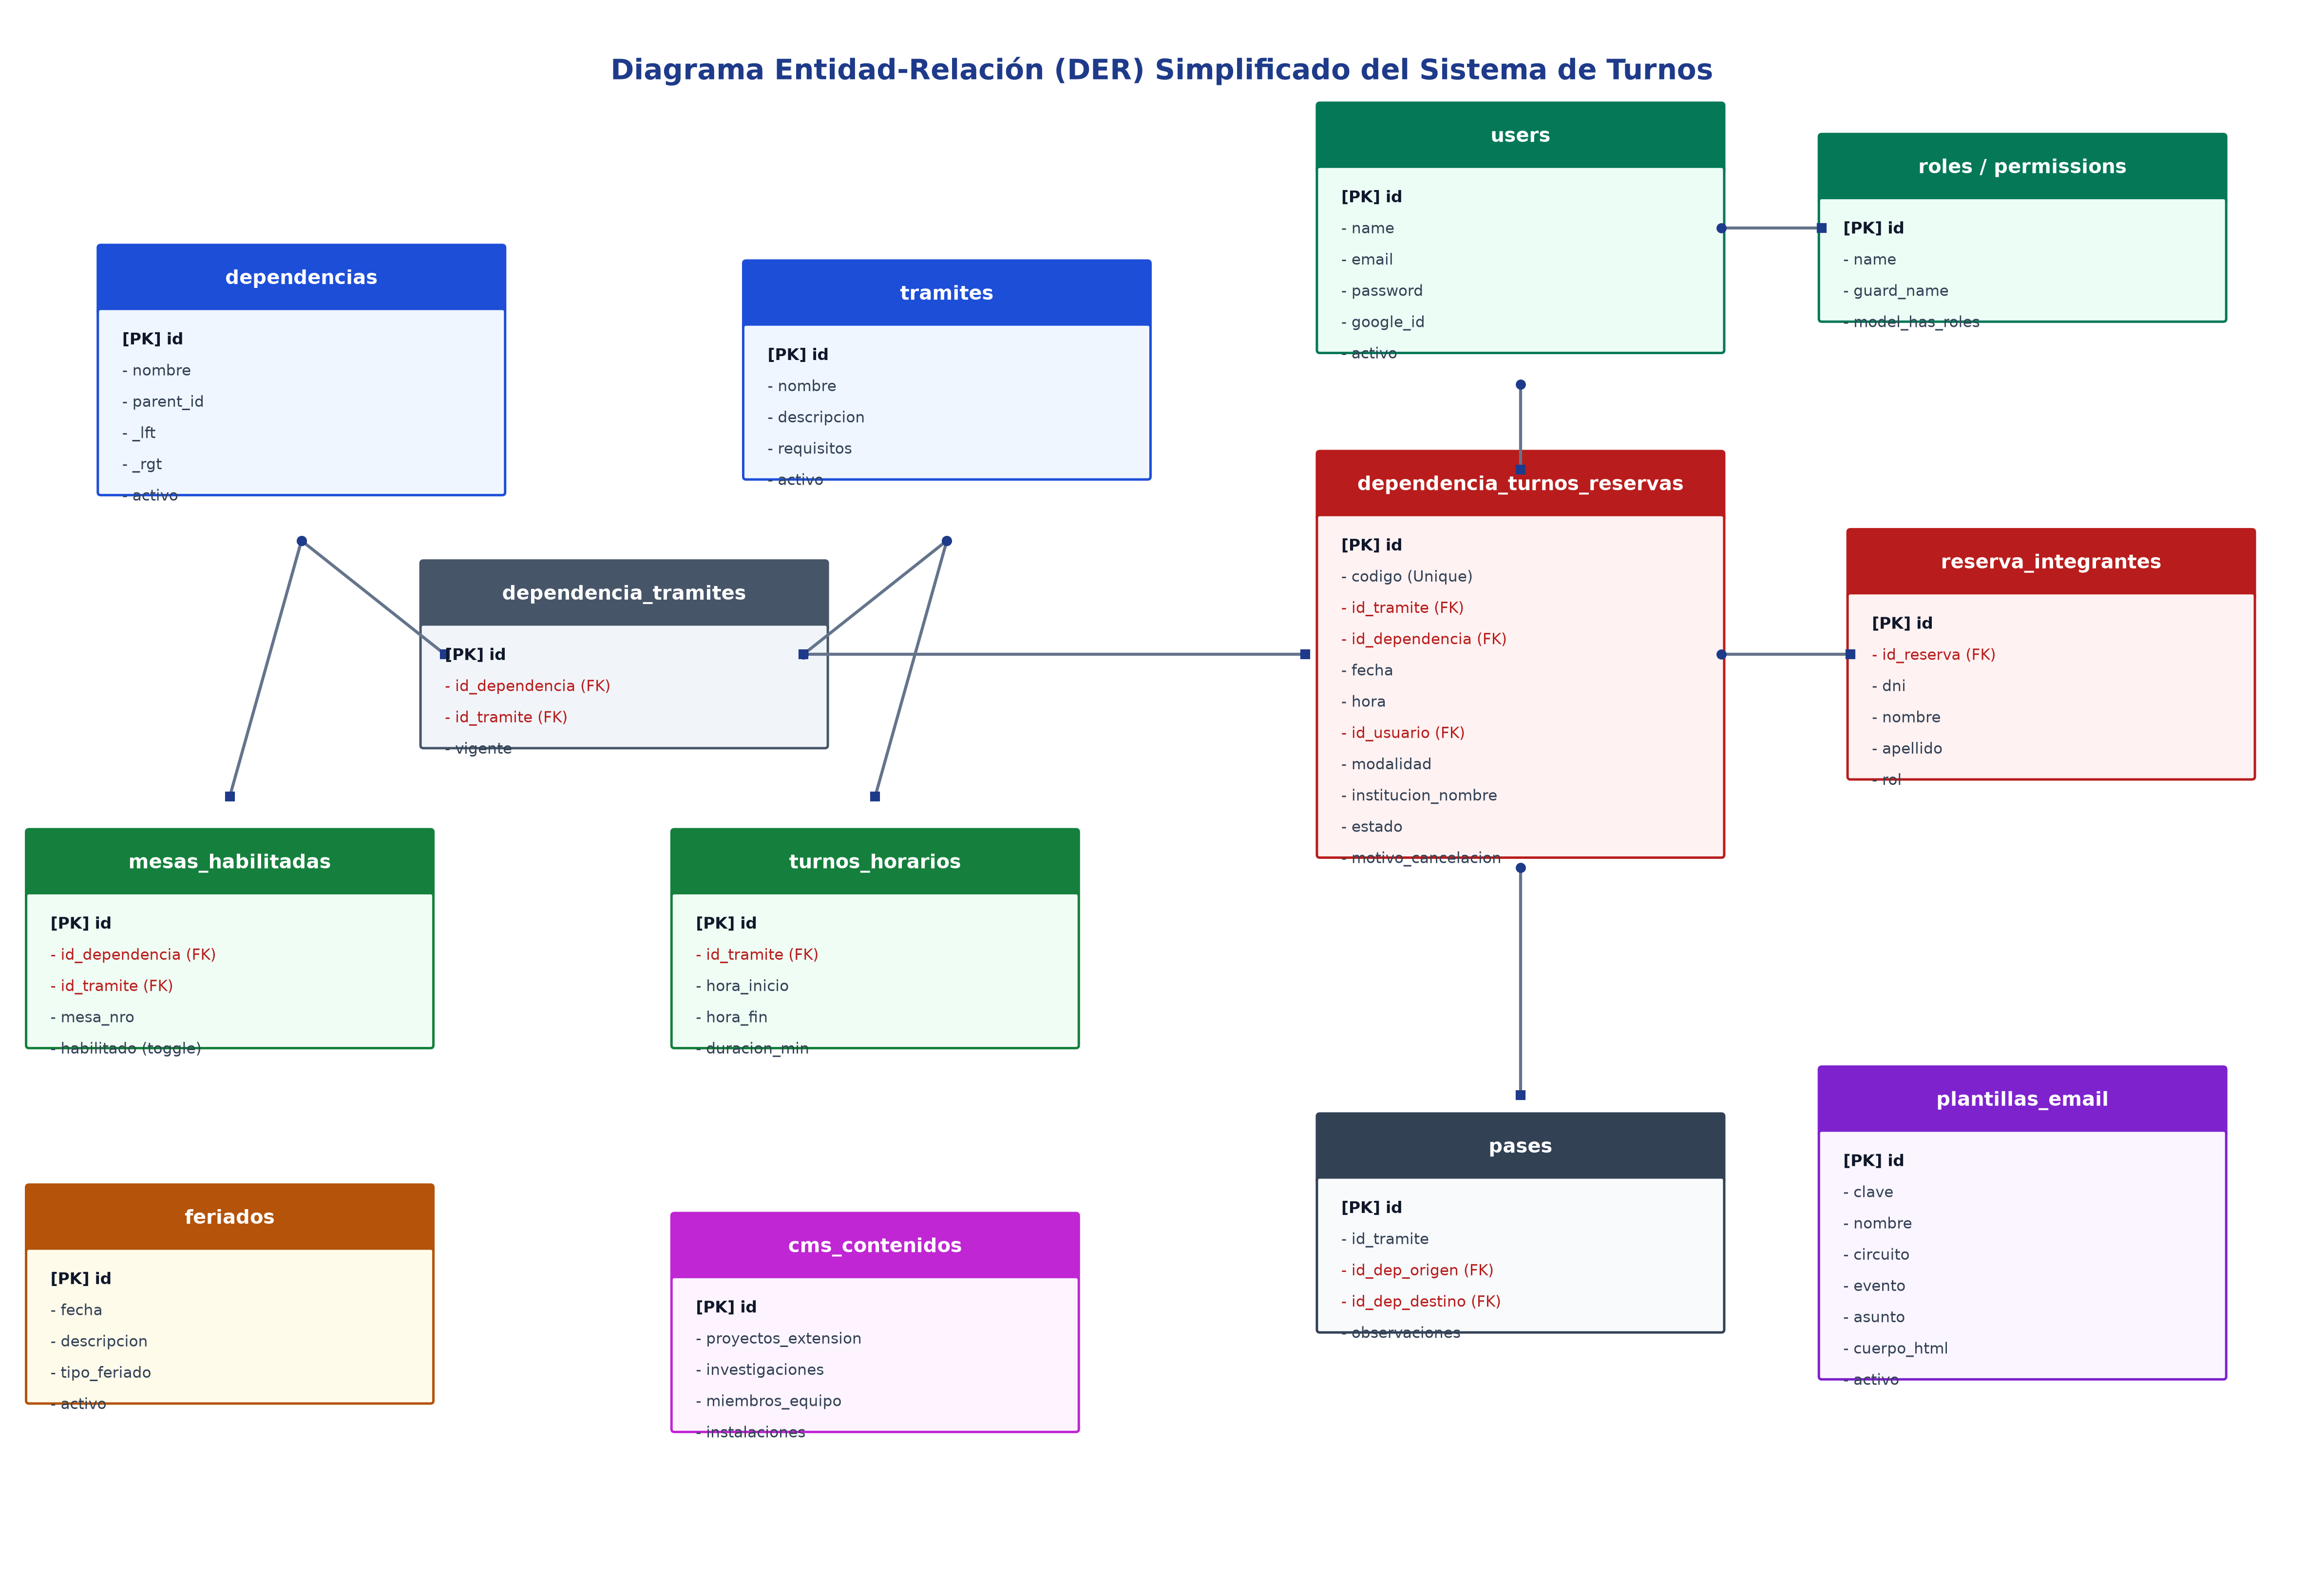
\includegraphics[width=0.95\textwidth]{diagrama_er}
    \caption{Diagrama Entidad-Relación (DER) simplificado del sistema de turnos}
    \label{fig:diagrama_er}
\end{figure}

\begin{itemize}
    \item \textbf{Dependencias y Jerarquía:} La tabla \texttt{dependencias} es la columna vertebral del sistema. Utiliza el motor \textit{InnoDB} para soportar claves foráneas. La implementación del patrón \textbf{Nested Set} (\texttt{\_lft}, \texttt{\_rgt}) permite realizar consultas jerárquicas rápidas, fundamental para representar la estructura UNSa $\rightarrow$ Facultad $\rightarrow$ Departamento $\rightarrow$ Observatorio.
    \item \textbf{Gestión de Trámites y Asignaciones:} La entidad \texttt{tramites} almacena el catálogo de actividades. La relación con las dependencias se gestiona a través de \texttt{dependencia\_tramites}, permitiendo que una dependencia específica (como el Observatorio) ofrezca un conjunto particular de servicios. A su vez, \texttt{usuarios\_dependencias} asocia operadores con sus respectivas dependencias para asegurar la segregación de información.
    \item \textbf{Reservas de Turnos y Nóminas de Asistentes:} La tabla \texttt{dependencia\_turnos\_reservas} centraliza las citas solicitadas (código alfanumérico, datos del titular, fecha, franja horaria, estado y motivos de cancelación). Para soportar delegaciones escolares e institucionales, se vincula con la tabla \texttt{reserva\_integrantes}, donde se almacena la nómina detallada de estudiantes y acompañantes con sus respectivos números de documento.
    \item \textbf{Capacidad Operativa y Horarios:} Las tablas \texttt{turnos\_horarios} y \texttt{mesas\_habilitadas} definen los bloques horarios por trámite y regulan la capacidad simultánea de atención. La tabla \texttt{mesas\_habilitadas} incluye el campo de activación rápida para habilitar o suspender puestos según el personal de turno.
    \item \textbf{Gestión de Plantillas de Correo Transaccional:} La tabla \texttt{plantillas\_email} almacena las definiciones HTML de las comunicaciones. Incluye columnas para la clave identificadora, nombre, circuito operativo (\textit{individual} o \textit{colegio}), evento disparador (\textit{solicitud}, \textit{confirmacion}, \textit{cancelacion}), asunto con placeholders, cuerpo HTML, listado de variables dinámicas disponibles y estado activo/inactivo.
    \item \textbf{Calendario y Días No Laborables:} La tabla \texttt{feriados} registra las fechas festivas y asuetos institucionales, permitiendo al motor de reservas excluir dichas jornadas de forma desatendida.
    \item \textbf{Trazabilidad de Derivaciones:} La tabla \texttt{pases} registra el historial de expedientes y trámites de solicitantes derivados entre dependencias, asentando las dependencias intervinientes, observaciones y fecha de emisión.
    \item \textbf{Gestor de Contenidos Institucionales (CMS):} Se integran las tablas \texttt{proyectos\_extension}, \texttt{investigaciones}, \texttt{miembros\_equipo}, \texttt{instalaciones} y \texttt{tipos\_evento}, las cuales estructuran los recursos de divulgación científica exhibidos en el portal público del Observatorio.
\end{itemize}

\section{Diccionario de Datos y Migraciones}
La estructura se ha implementado utilizando las \textbf{Migraciones de Laravel}, lo que permite un control de versiones preciso sobre el esquema de la base de datos y su recreación reproducible en cualquier entorno.

\begin{figure}[htbp]
    \centering
    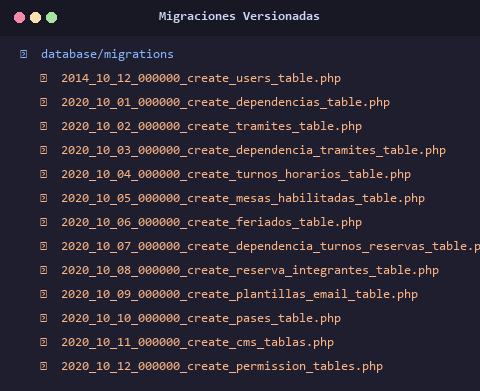
\includegraphics[width=0.55\textwidth]{codigo_tree_migrations}
    \caption{Historial versionado de migraciones de la base de datos en \texttt{database/migrations/}}
    \label{fig:tree_migrations}
\end{figure}

Entre los tipos de datos y restricciones más relevantes se destacan:

\begin{itemize}
    \item \textbf{Tipos de Datos Optimistas:} Se utilizan campos de tipo \texttt{tinyint(1)} para estados booleanos (activo/inactivo), optimizando el almacenamiento.
    \item \textbf{Integridad Referencial:} Se han definido restricciones \texttt{ON DELETE CASCADE} en tablas críticas como las de roles y permisos (\texttt{model\_has\_roles}), asegurando que no existan registros huérfanos.
    \item \textbf{Trazabilidad:} Todas las tablas incluyen los campos \texttt{created\_at} y \texttt{updated\_at}, permitiendo auditar cuándo se creó una dependencia o cuándo se modificó el estado de un turno.
\end{itemize}

\section{Optimización y Rendimiento}
Debido a que el sistema puede recibir una alta concurrencia durante periodos de inscripciones o eventos en el Observatorio, se han aplicado las siguientes estrategias:

\begin{itemize}
    \item \textbf{Indexación Estratégica:} Se han creado índices compuestos, como en la tabla \texttt{dependencias} (\texttt{\_lft}, \texttt{\_rgt}, \texttt{parent\_id}), para acelerar la navegación por el árbol académico.
    \item \textbf{Soft Deletes:} Tablas como \texttt{personas} y \texttt{dependencias} implementan \textit{borrado lógico} (\texttt{deleted\_at}), permitiendo recuperar información eliminada accidentalmente y manteniendo el historial de atención.
\end{itemize}
